\documentclass[12pt]{article}\usepackage{indentfirst}\usepackage[margin=2cm]{geometry}
\usepackage{graphicx}
 
\begin{document}
	\title{\Huge{Rapport TP ANI-IA 4068}}\author{Claude Rene EZOM AIA 4}\date{5$^{th}$ Mars 2024}\maketitle\tableofcontents\newpage
	\section{INTRODUCTION}
	La programmation informatique est une discipline indispensable dans la
  conception logicielle. Pour mieux asseoir ses bases dans cette discipline, il est capital de s'exercer à la programmation des jeux vidéos. Notre étude se focalisera uniquement sur la production 
  d'une application événementielle base sur la bibliothèque Pygame du langage de programmation Python.
  \section{PRÉSENTATION}
	 A travers cette étude, il est question pour nous de concevoir
  une application permettant de détecter une touche enfoncée sur le clavier d'un ordinateur puis afficher le résultat sur l'écran à travers une fenêtre générée par la bibliothèque PYGAME du langage de programmation Python.

 \section{DÉMONSTRATION}
	\subsection{Création de la fenêtre et affichage}
    \begin{minipage}{0.49\textwidth}
    \centering
    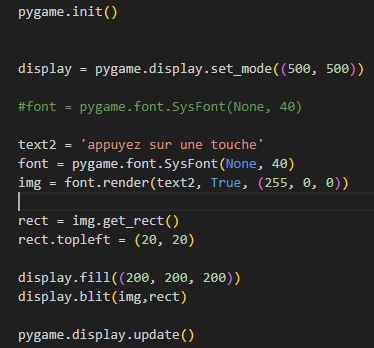
\includegraphics[width=1\textwidth]{Images/2.png}
    \caption{Expérimentation}
    \label{fig:1}
    \end{minipage}
    \hfill
    \begin{minipage}{0.49\textwidth}
    \centering
    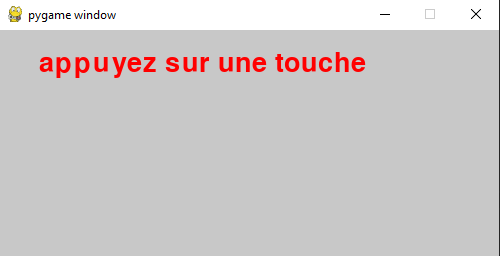
\includegraphics[width=1\textwidth]{Images/3.png}
    \caption{résultat}
    \label{fig:2}
    \end{minipage}.
    \subsection{Gestion des évènements et testes}
    \begin{minipage}{0.49\textwidth}
    \centering
    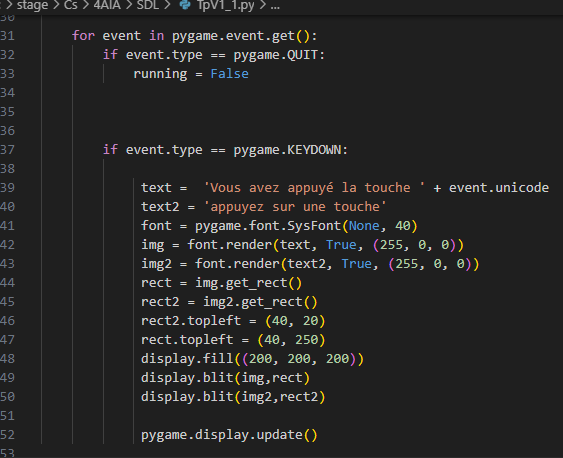
\includegraphics[width=1\textwidth]{Images/4.png}
    \caption{Expérimentation2}
    \label{fig:1}
    \end{minipage}
    \hfill
    \begin{minipage}{0.49\textwidth}
    \centering
    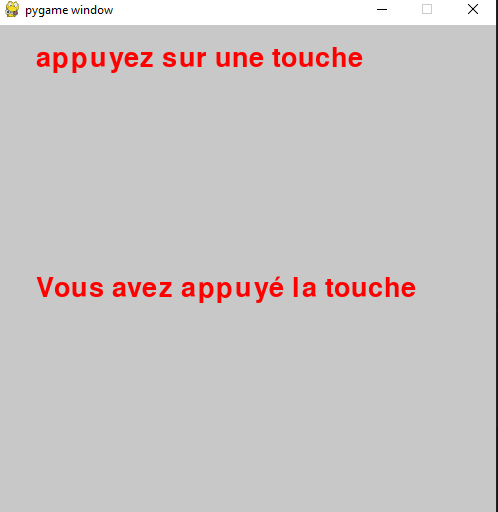
\includegraphics[width=1\textwidth]{Images/5.png}
    \caption{teste}
    \label{fig:2}
    \end{minipage}.
    
	
\end{document}